\ChapterImageStar[cap:pmv]{Producto Mínimo Viable }{./images/fondo.png}\label{cap:pmv}
\mbox{}\\
\section{Código fuente del sistema}
\noindent
El código fuente del sistema, desarrollado en el lenguaje Bash, está disponible en el repositorio de GitHub \href{https://github.com/AariazP/TG-VBC.git}{\texttt{TG-VBC}} en la rama \texttt{scripted-solution}. Este repositorio contiene scripts para la automatización de tareas en la infraestructura de virtualización basada en contenedores, incluyendo la configuración de nodos, despliegue de \VM\ y configuración de Kubernetes. 
La figura~\ref{fig:estructura-proyecto} detalla la estructura del proyecto
\begin{figure}[H]
    \centering
    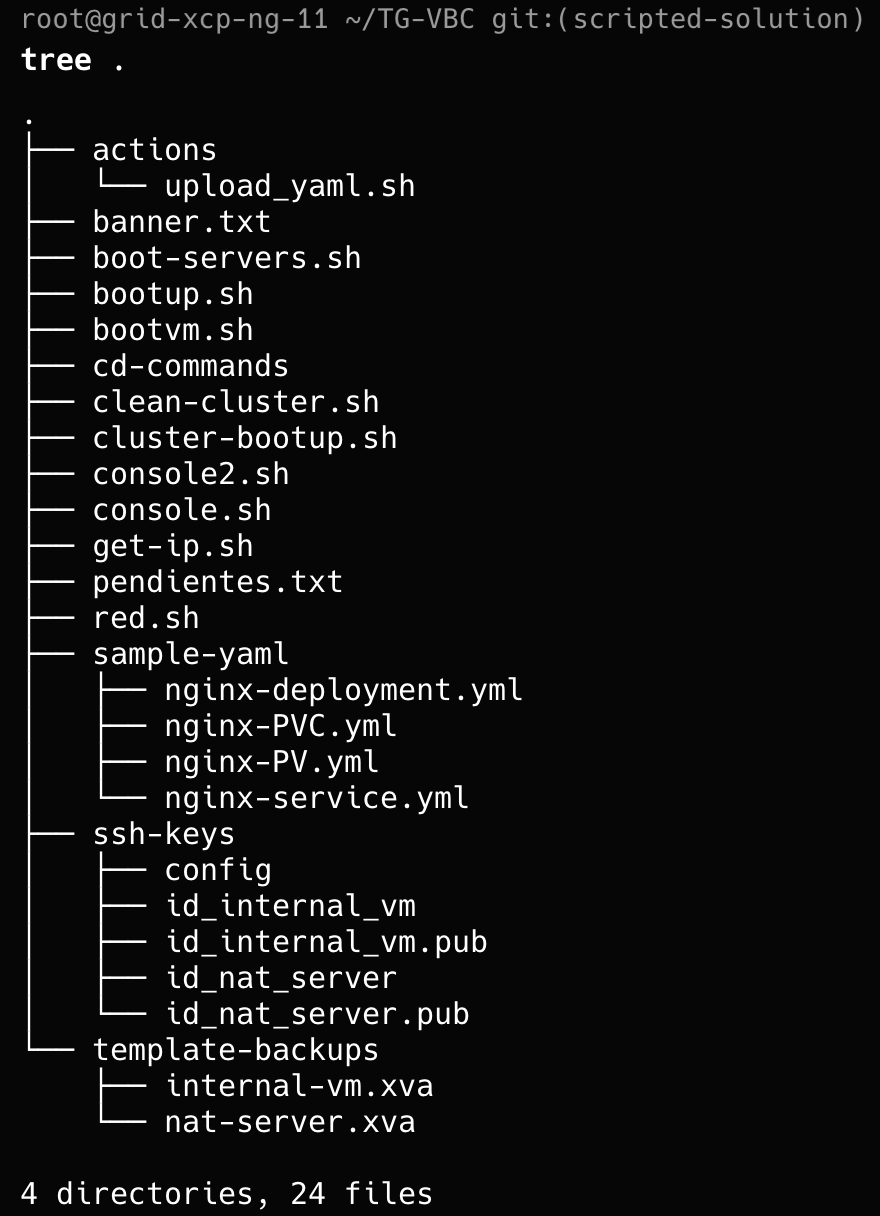
\includegraphics[scale=0.2]{tablas-images/cp6/src/tree.png}
    \caption{Estructura del proyecto}\label{fig:estructura-proyecto}
\end{figure}

\subsection{Script para obtener la IP de una VM en XCP-ng}
\noindent
El \textit{script}~\ref{fig:get-ip}, construido en Bash tiene como propósito obtener la dirección IP asociada a una \VM\ desplegada en un entorno XCP-ng, a partir de su nombre. En primer lugar, valida que el usuario haya proporcionado al menos un argumento, correspondiente al nombre de la \VM, mostrando un mensaje de uso en caso contrario. Posteriormente, contempla una excepción para la máquina denominada \textit{NAT-Master}, devolviendo directamente la IP fija 172.30.29.2. En los demás casos, el script emplea el comando xe para obtener el identificador único (UUID) de la máquina virtual y, a partir de este, extrae las direcciones \MAC\ de sus interfaces de red. Con dichas direcciones, se conecta mediante \SSH\ a la máquina \textit{NAT-Master}, utilizando una clave previamente configurada, y consulta la tabla de vecinos de red (comando ip n) para identificar la IP correspondiente a las \MAC\ recuperadas. Finalmente, devuelve la dirección IP asociada a la \VM\ solicitada.

\begin{minted}[frame=lines,fontsize=\footnotesize,breaklines]{bash}
#!/bin/bash

# ---------------------------------------------------------------
# Script: get-ip.sh
# Descripción:
#   Este script obtiene la dirección IP de una máquina virtual 
#   (VM) en XCP-ng a partir de su nombre.
# ---------------------------------------------------------------

# Verificación de argumentos:
# Si no se pasa al menos un argumento (nombre de la VM), se muestra 
# el uso correcto del script y se termina.
if [ $# -lt 1 ]
then
   echo "usage: get-ip <vm-name>"
   exit 0
fi

# Caso especial: 
# Si el nombre de la VM es "NAT-Master", se devuelve una IP fija 
# sin necesidad de consultar nada en XCP-ng.
if [[ "$1" == "NAT-Master" ]]
then
   echo "172.30.29.2"
   exit 0
fi

# Obtiene el UUID de la VM en XCP-ng a partir del nombre de la VM.
VM_UUID=$( xe vm-list name-label="$1" --minimal )

# Obtiene las direcciones MAC de las interfaces de red (VIFs) 
# asociadas a la VM, separadas por coma.
VM_MAC=$( xe vif-list vm-uuid="$VM_UUID" params=MAC --minimal )

# Convierte la lista separada por comas en un arreglo de MACs. 
# Se asumen máximo dos interfaces de red.
MACS=( $( echo $VM_MAC | cut -d, -f1 ) $( echo $VM_MAC | cut -d, -f2 ) )

# Redirige los errores a /dev/null para evitar mostrar mensajes 
# de advertencia de ssh u otros.
exec 2> /dev/null

# Se conecta al servidor NAT (172.30.29.2) vía SSH usando una llave 
# privada, y ejecuta el comando `ip n` (vecinos en ARP/NDP).
# Luego filtra las líneas que contengan alguna de las MACs de la VM 
# y extrae la primera columna (la IP asociada).
VM_IP=$( ssh -i ~/.ssh/id_nat_server debian@172.30.29.2 \
        "ip n | fgrep -e ${MACS[0]} -e ${MACS[1]}" | cut -d" " -f1 )

# Muestra la IP obtenida sin salto de línea adicional al final.
echo -n $VM_IP

\end{minted}

\begin{figure}[H]
    \centering
    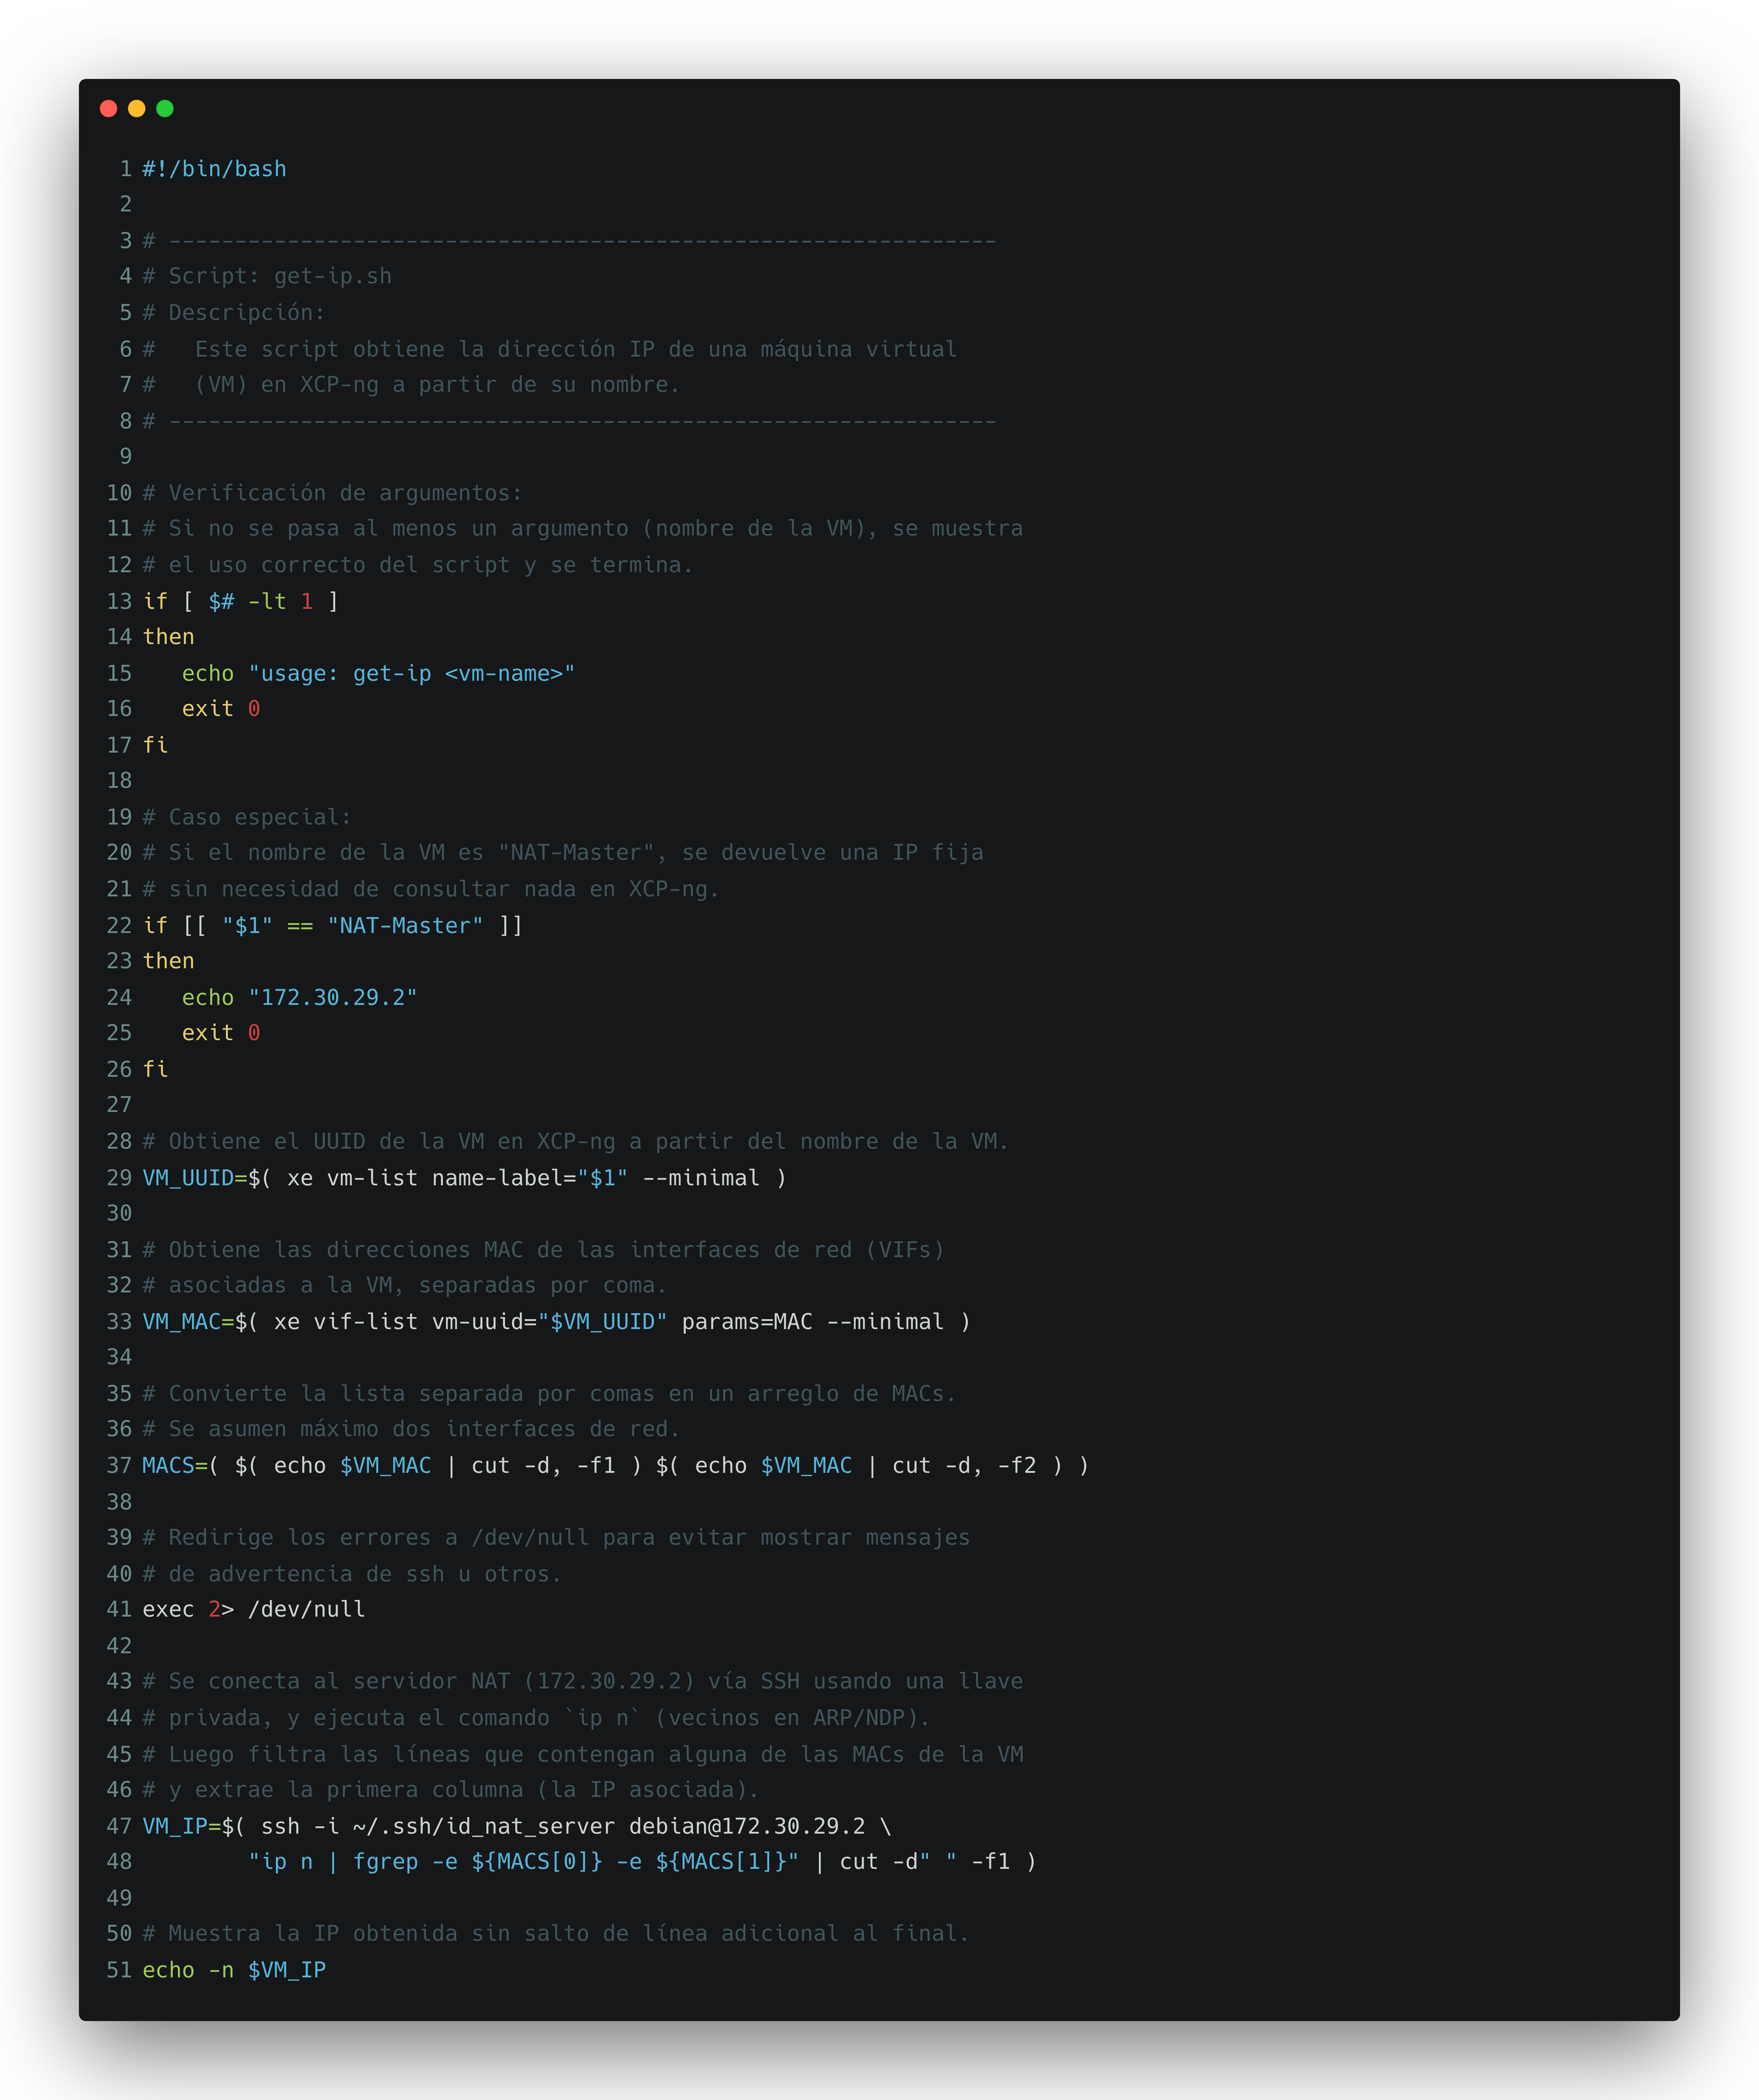
\includegraphics[width=\textwidth]{tablas-images/cp6/src/get-ip.png}
    \caption{Script que obtiene la IP de una VM en XCP-ng}\label{fig:get-ip}
\end{figure}

\subsection{Script de configuración de red de las VMs}
\noindent
El \textit{script}~\ref{fig:configure-network} automatiza la creación y configuración de una red virtual en un entorno XCP-ng, permitiendo la salida a Internet para las máquinas virtuales que se conecten a ella. En primer lugar, define parámetros como el nombre de la red, el rango de direcciones IP (subred), la dirección de la puerta de enlace y la interfaz de salida hacia Internet. Luego, utiliza el comando \texttt{xe network-create} para crear la red virtual sin necesidad de un \textit{bridge} preexistente y obtiene su UUID para validarla. Una vez confirmada la red, se agrega una interfaz virtual al host con una dirección \MAC\ aleatoria. Posteriormente, se asocia al bridge correspondiente la dirección IP de la puerta de enlace definida y se activa la interfaz.
\noindent
El \textit{script} también habilita el reenvío de paquetes IP, tanto de forma temporal como persistente en el archivo de configuración del sistema, lo que permite que el host actúe como enrutador. Seguidamente, configura reglas de \NAT\ con iptables, aplicando enmascaramiento para que las máquinas virtuales dentro de la subred puedan acceder a Internet a través de la interfaz física de salida del \textit{host}. Finalmente, contempla la persistencia de estas reglas con herramientas como \texttt{netfilter-persistent}.
\begin{figure}[H]
    \centering
    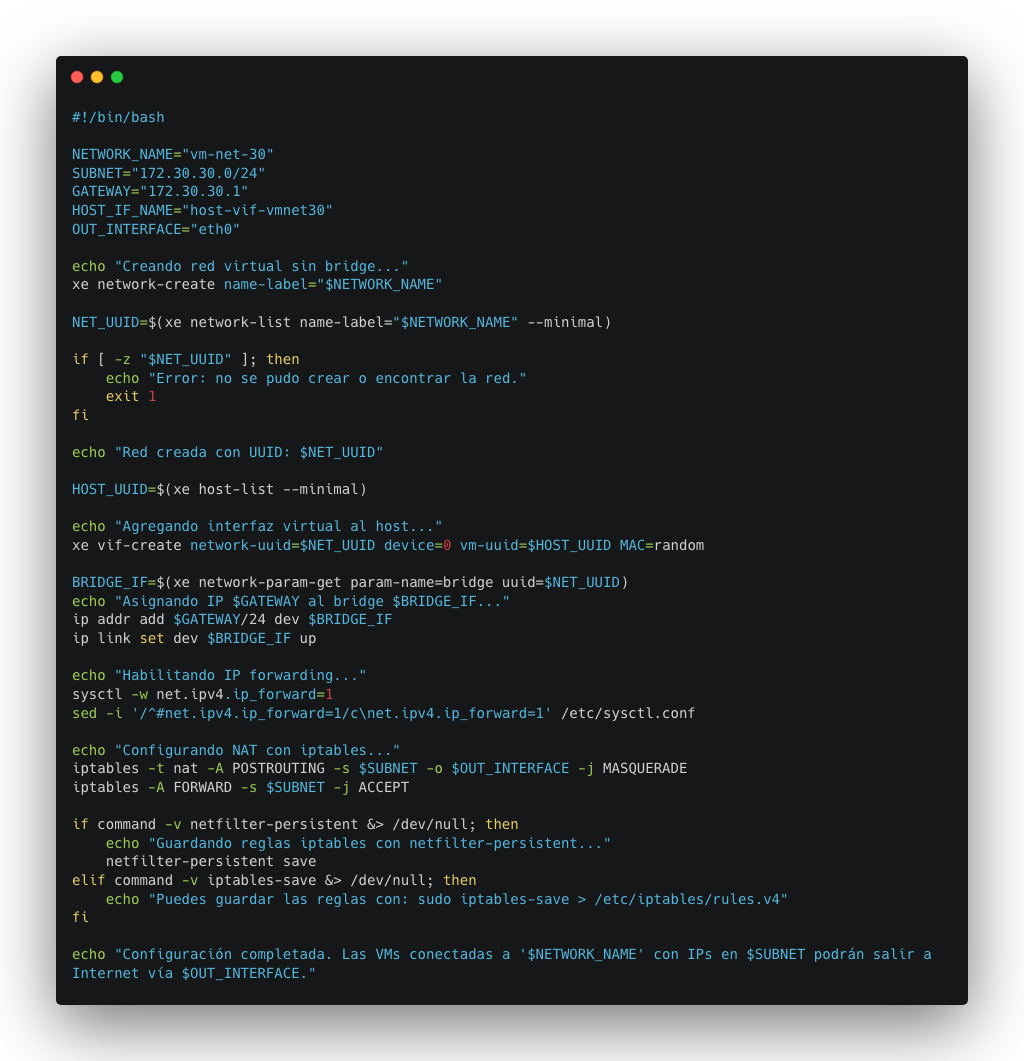
\includegraphics[width=\textwidth]{tablas-images/cp6/src/red.png}
    \caption{Script que configura la red de las VMs}\label{fig:configure-network}
\end{figure}

\subsection{Script de conexión SSH a una VM}
\noindent
El script~\ref{fig:sshvm} tiene como propósito facilitar la conexión remota por medio de \SSH\ a las diferentes \VM\ dentro de un entorno administrado, ofreciendo además la posibilidad de ejecutar comandos de forma directa en ellas. Su funcionamiento se puede dividir en las siguientes fases:

\begin{enumerate}
    \item \textbf{Parámetros de entrada}:  
    El script admite dos opciones principales:
    \begin{itemize}
        \item \texttt{-r}: establece que la conexión debe realizarse como el usuario \texttt{root}.
        \item \texttt{-c <comando>}: permite especificar un comando a ejecutar directamente en la máquina virtual, en lugar de iniciar una sesión interactiva.
    \end{itemize}
    Además, es obligatorio proporcionar el nombre de la VM como argumento principal.

    \item \textbf{Procesamiento de opciones}:  
    Se emplea el comando \texttt{getopts} para interpretar los parámetros recibidos. En caso de que los argumentos no cumplan con el formato esperado, se muestra un mensaje de uso correcto y el programa termina.

    \item \textbf{Resolución de la dirección IP de la VM}:  
    A través de la función auxiliar \texttt{get-ip}, el script obtiene la dirección IP asociada a la máquina virtual especificada. Los mensajes de error se redirigen a \texttt{/dev/null} para mantener una salida limpia.

    \item \textbf{Conexión mediante SSH}:  
    Existen dos escenarios:
    \begin{itemize}
        \item Si se activó la opción \texttt{-r}, la conexión se establece como el usuario \texttt{root}, utilizando una clave privada almacenada en \texttt{\~{}/.ssh/id\_internal\_vm}.
        \item En caso contrario, la conexión se realiza con el usuario por defecto, sin especificar clave adicional.
    \end{itemize}
    En ambos casos, si se definió un comando con la opción \texttt{-c}, este será ejecutado de inmediato en la máquina virtual. De lo contrario, se abrirá una sesión \SSH\ interactiva.

\end{enumerate}

\begin{figure}[H]
    \centering
    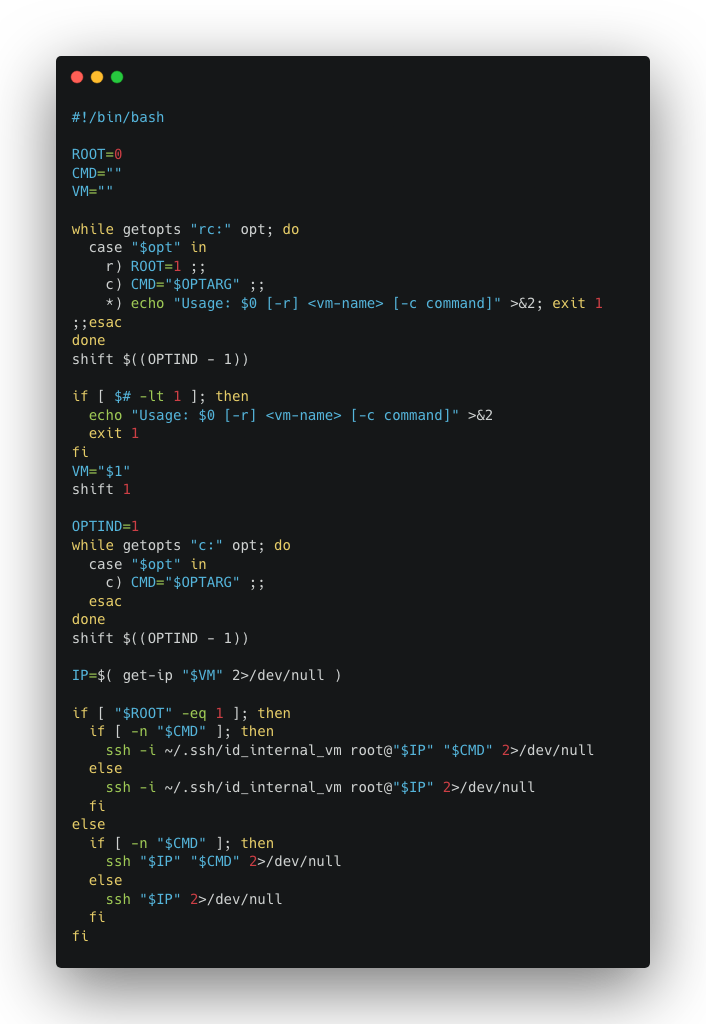
\includegraphics[width=\textwidth]{tablas-images/cp6/src/ssh-vm.png}
    \caption{Script que permite la conexión SSH a una VM}\label{fig:sshvm}
\end{figure}

\subsection{Script de configuración inicial de una VM}

\subsection{Explicación del script \texttt{bootup.sh}}

El script \texttt{bootup.sh} fue diseñado para desplegar y configurar máquinas virtuales en XCP-ng de forma manual, en un contexto anterior a la creación de plantillas predefinidas. Aunque actualmente no se utiliza de manera habitual, se conserva como alternativa en caso de que las plantillas se pierdan o deba realizarse una instalación manual. A continuación, se detallan sus principales fases de ejecución:

\begin{enumerate}
    \item \textbf{Identificación del entorno}:  
    En primer lugar, el script lista los hosts disponibles mediante \texttt{xe host-list} y obtiene el UUID del host principal, exportándolo como variable de entorno. Posteriormente, muestra los repositorios de almacenamiento (SR) y las plantillas de sistema operativo, filtrando aquellas relacionadas con Debian.

    \item \textbf{Creación de la máquina virtual}:  
    Se define el nombre de la VM (por defecto \texttt{xeclivm} si no se pasa argumento) y se crea una nueva instancia a partir de la plantilla \texttt{Debian Bookworm 12}. A continuación, se obtiene el UUID de la VM recién creada para su uso posterior.

    \item \textbf{Gestión de medios de instalación}:  
    Se prepara un directorio local para almacenar imágenes ISO, se crea un SR de tipo ISO y se obtiene su UUID. Tras forzar un escaneo de dicho repositorio, se selecciona el archivo ISO de instalación de Debian que se utilizará para la instalación de la VM.

    \item \textbf{Configuración de almacenamiento y red}:  
    El script localiza el disco virtual asociado a la VM y lo redimensiona a 20~GiB. Asimismo, identifica el UUID de la red principal (\texttt{xenbr0}) y crea una interfaz de red para la máquina virtual.

    \item \textbf{Parámetros de hardware y arranque}:  
    Se configuran los límites de memoria de la VM (mínimos y máximos) y la política de arranque mediante BIOS. También se desactiva \textit{Secure Boot}, se fuerza el modelo tradicional de QEMU y se definen los dispositivos de arranque (disco y CD).  

    \item \textbf{Gestión de dispositivos de CD-ROM}:  
    Se expulsan posibles medios previos y se insertan las ISOs necesarias, incluyendo tanto \texttt{guest-tools.iso} como la ISO de Debian especificada. Esto asegura que la VM disponga de los medios de instalación y herramientas complementarias.

    \item \textbf{Inicio de la máquina virtual}:  
    Finalmente, la VM se arranca utilizando el UUID generado durante su creación, completando el proceso de despliegue.

\end{enumerate}

En conjunto, este script constituye una solución integral para la creación de máquinas virtuales en XCP-ng sin depender de plantillas predefinidas, abarcando desde la preparación de medios de instalación hasta la configuración de red, almacenamiento, parámetros de arranque y el inicio de la máquina virtual.

\begin{figure}[H]
    \centering
    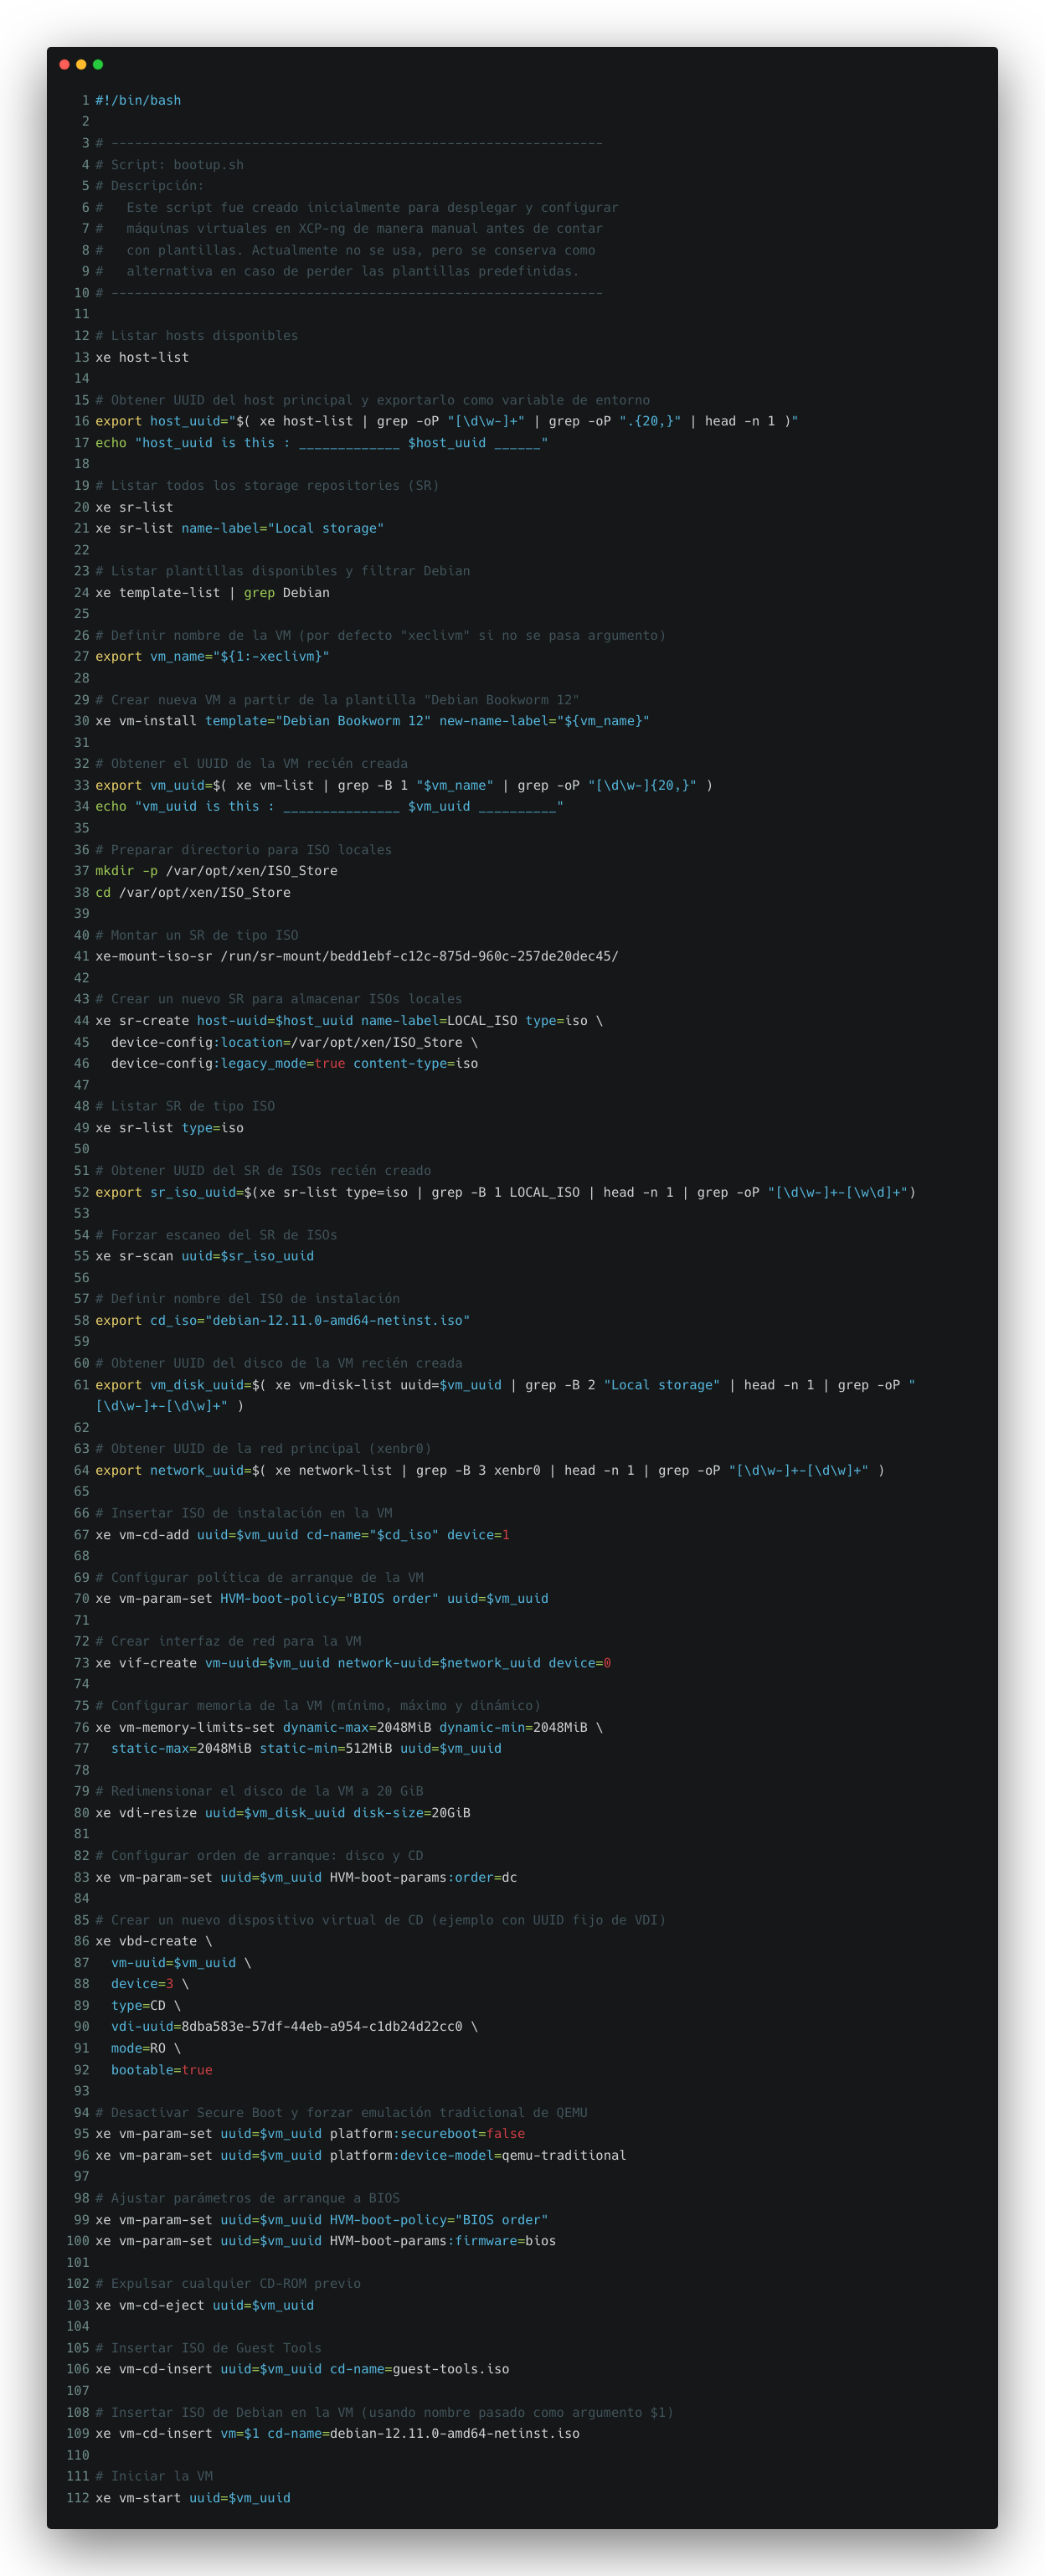
\includegraphics[scale=0.2]{tablas-images/cp6/src/bootup-vm.png}
    \caption{Script que permite la configuración inicial de una VM}\label{fig:bootup-vm}
\end{figure}
